\documentclass[twocolumn,landscape,10pt]{article}
\usepackage[thinc]{esdiff} % for typesettign derivatives
\usepackage{amsthm} % provides an enhanced version of LaTex's \newtheorem command
\usepackage{mdframed} % framed environments that can split at page boundaries
\usepackage{enumitem} % bulletin points or other means of listing things
\usepackage{amssymb} % for AMS symbols
\usepackage{amsmath} % so as to use align
\usepackage{latexsym} % so as to use symbols like \leadsto
\usepackage{mathrsfs} % for using mathscr for char like operators
\usepackage{commath} % for using norm symbol
\usepackage{mathtools} % for using environments like dcases
\usepackage{authblk} % for writing affiliations
\usepackage{graphicx} % for importing images
\graphicspath{{./images/}} % for the path to images, also always put label behind captions
\usepackage{textcomp} % for using degree symbol
\usepackage{hyperref} % for clickable link in the pdf & customizable reference text
\usepackage[all]{hypcap} % for clickable link to images instead of caption
\usepackage[margin=1.0in]{geometry} % default is 1.5in
% \usepackage[left=0.4in, right=0.4in, top=0.8in, bottom=0.8in]{geometry}
\usepackage[title]{appendix} % for attaching appendix
\allowdisplaybreaks % allow page breaking in display maths, like align
\usepackage{xcolor} % for setting color of a block of text, use \textcolor{<color>}{}
\usepackage[normalem]{ulem} % for strikethrough text, use \sout{}
% allow for more advanced table layout
\usepackage{booktabs}
\usepackage{multirow}
\usepackage{siunitx}
% for adjusting caption settings
\usepackage{caption}
\captionsetup[table]{skip=10pt}

\theoremstyle{definition}
\mdfdefinestyle{defEnv}{%
  hidealllines=false,
  nobreak=true,
  innertopmargin=-1ex,
}

% The following is for writing block of code
\usepackage{listings}
\usepackage{color}

\definecolor{dkgreen}{rgb}{0,0.6,0}
\definecolor{gray}{rgb}{0.5,0.5,0.5}
\definecolor{mauve}{rgb}{0.58,0,0.82}

% setting of the thickness of the 4 lines of box
\setlength{\fboxrule}{2pt}

% Use the following to change code language and related settings
\lstset{frame=tb,
  language=Python,
  aboveskip=3mm,
  belowskip=3mm,
  showstringspaces=false,
  columns=flexible,
  basicstyle={\small\ttfamily},
  numbers=none,
  numberstyle=\tiny\color{gray},
  keywordstyle=\color{blue},
  commentstyle=\color{dkgreen},
  stringstyle=\color{mauve},
  breaklines=true,
  breakatwhitespace=true,
  tabsize=3,
  literate={~} {$\sim$}{1}
}

\pagestyle{headings}
\author{Lectured by Emil C Lupu}
\title{Distributed Systems}
\affil{Typed by Aris Zhu Yi Qing}
\begin{document}
\maketitle
\tableofcontents
\newpage

\section{Characteristics}

\subsection{Distribution Transparencies}

Realize a coherent system by \emph{hiding distribution} from the user where
possible.

\begin{itemize}
    \item \textbf{Access}: uniform access whether local or remote
    \item \textbf{Location}: access without knowledge of location
    \item \textbf{Concurrency}: sharing without interference (requires synchronization)
    \item \textbf{Replication}: hides use of redundancy (e.g. for fault tolerance)
    \item \textbf{Failure}: conceal failures by replication or recovery
    \item \textbf{Migration}: hides migration of components (e.g. for load balancing)
    \item \textbf{Performance}: hide performance variations (e.g. through use of
        scheduling and reconfiguration)
    \item \textbf{Scaling}: permits expansion by adding more resources (e.g. cloud)
\end{itemize} 

\subsection{Challenges}

\begin{itemize}
    \item \textbf{Heterogeneity}: different OS, data
        representation, implementations, etc.
    \item \textbf{Openness}: need to define \emph{interfaces} for components to
        easily scale up systems
    \item \textbf{Security}: control access to preserve integrity and
        confidentiality
    \item \textbf{Concurrency}: inconsistencies may arise with interleaving
        requests
    \item \textbf{Failure handling}: transient/permanent failures could occur at
        any time. It is difficult detect them and to maintain consistency.
    \item \textbf{Scalability}: size of the system makes it difficult to
        maintain information about \emph{system state}.
\end{itemize} 

\subsection{Wrong Assumptions}

\begin{itemize}
    \item The network is reliable, secure \& homogeneous.
    \item The topology does not change.
    \item The latency is zero.
    \item The bandwidth is infinite.
    \item Transport cost is zero.
    \item There is one administrator.
\end{itemize} 

\subsection{Terminology}

\begin{itemize}
    \item \textbf{Client}: an entity initiating an interation
    \item \textbf{Server}: a componenet responds to interactions usually
        implemented as a process
    \item \textbf{Service}: a componenet of a computer system that manages a
        collection of resources and presents their functionality to users.
    \item \textbf{Middleware}: software layer between the application and the OS
        masking the heterogeneity of the underlying system.
\end{itemize} 


\section{Architecture}

\subsection{Layered architecture}
\begin{itemize}
    \item e.g. Network stack. Control flows downwards, results flow upwards.
    \item[+] framework is simple and easy to learn and implement
    \item[+] reduced dependency due to layer separation
    \item[+] testing is easier with such modularity
    \item[+] cost overheads are fairly low
    \item[-] scalability is difficult due to fixed framework structure
    \item[-] difficult to maintain, since a change in a single layer can
        affect the entire system because it operates as a single unit
    \item[-] parallel processing is not possible
\end{itemize} 

\subsection{Object-based and service-oriented architectures}
\begin{itemize}
    \item e.g. RMI
    \item[+] reusability, easy maintainability and greater reliability
        due to modularity
    \item[+] improved scalability and availability: multiple instances
        of a single service can run on different servers at the same
        time.
    \item[-] Increased overhead: Service interactions require
        validations of inputs, thereby increasing the response time and
        machine load, and reducing the overall performance
\end{itemize} 

\subsection{Message-based architectures}
\begin{table}[h]
    \centering
    \begin{tabular}{ll||c|c}
          & & Temporally coupled & Temporally decoupoled \\
        \hline\hline
        \rule{0pt}{20px} &
        \shortstack{Referentially \\coupled} & Direct process messaging & Messaging via
        mailbox \\
        \hline
        \rule{0pt}{20px} &
        \shortstack{Referentially \\decoupled} & Event-based (publish-subscribe) &
        Shared data spaces \\
    \end{tabular} 
\end{table} 
\begin{itemize}
    \item \underline{\emph{Referentially coupled}}: processes name
        sender/receiver in their communication.
    \item \underline{\emph{Temporally coupled}}: both sender and receiver need
        to be up and running.
\end{itemize} 

\subsection{Peer-to-peer}
\begin{itemize}
    \item structured: Each node is indexed so that the location is
        known, and messages are routed according to the topology.
    \item unstructured: \emph{flooding} or \emph{random walks} or both.
    \item[+] no server needed since individual workstations are used to
        access files
    \item[+] resilient to computer failures, since it does not disrupt
        any other part of the network
    \item[+] very scalable
    \item[-] poor performance with larger networks since each computer is being
        accessed by other users
    \item[-] no central file system, hard to look up or backup
    \item[-] ensuring that viruses are not introduced into the network
        is the responsibility of each individual user.
    \item[-] There is no security other than assigning permissions.
\end{itemize} 

\section{Message-passing and IPC}

\begin{itemize}
    \item \underline{Asynchronous send}: sender continues its execution once the
        message has been copied out of its address space
        \begin{itemize}
            \item[+] mostly used with \emph{blocked receive}
            \item[+] underlying system must provide buffering for receiving
                messages independently of receiver processes
            \item[+] \emph{loose} coupling: sender does not know when message will
                be received, does not suspend execution until the message has
                been received
            \item[-] \emph{Buffer exhaustion} (no flow control)
            \item[-] formal verification is more difficult, as need to account
                for the state of the buffers
        \end{itemize} 
    \item \underline{Synchronous send}: \emph{blocked send}, where the sender
        is held up until actual receipt of the message by the destination.
        \begin{itemize}
            \item[+] usually used with blocking receive, where receiver
                execution is suspended until a message is received.
            \item[+] synchronization between sender and receiver
            \item[+] generallyl easier to formally reason about synchronous
                systems
            \item[-] what if no receivers? message loss?
            \item[-] No multi-destination, requiring synchronization with all
                receivers.
            \item[-] implementation more complicated
            \item[-] The underlying communication service is expected to be
                \emph{reliable}, i.e.\ to guarantee in order message delivery.
        \end{itemize} 
    \item \underline{Asynchronous receive}: process continues execution if there
        are no messages. hardly provided as primitives
    \item \underline{Blocked receive}: the destination process blocks if no
        message is available, and receives it into a target variable when
        available.
    \item Please check the coursework for how UDP client/server is implemented in Java, 
        e.g. how datagram, socket, port are used.
\end{itemize} 

\section{Complex Data Representation}

\subsection{Definition}

\begin{itemize}
    \item \textbf{Marshalling} takes a collection of data items and transform
        them in a format suitable for transmission.
    \item \textbf{Unmarshalling} reconstitutes the data values and data
        structures from the bytes received.
\end{itemize} 

\subsection{Encoding structures}

\begin{figure}[h]
  	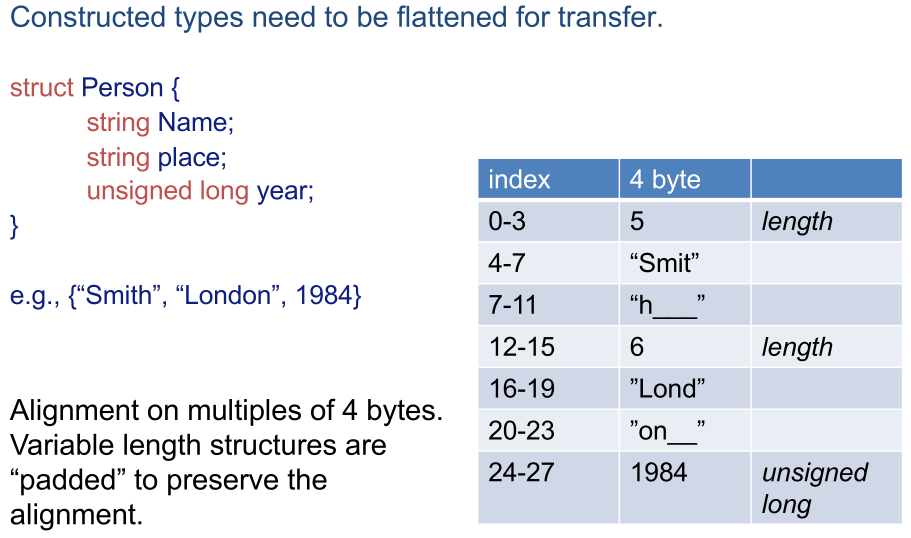
\includegraphics[scale=0.35]{encode_struct.png}
  	\centering
\end{figure}

\subsection{Composed structures}

\begin{figure}[h]
  	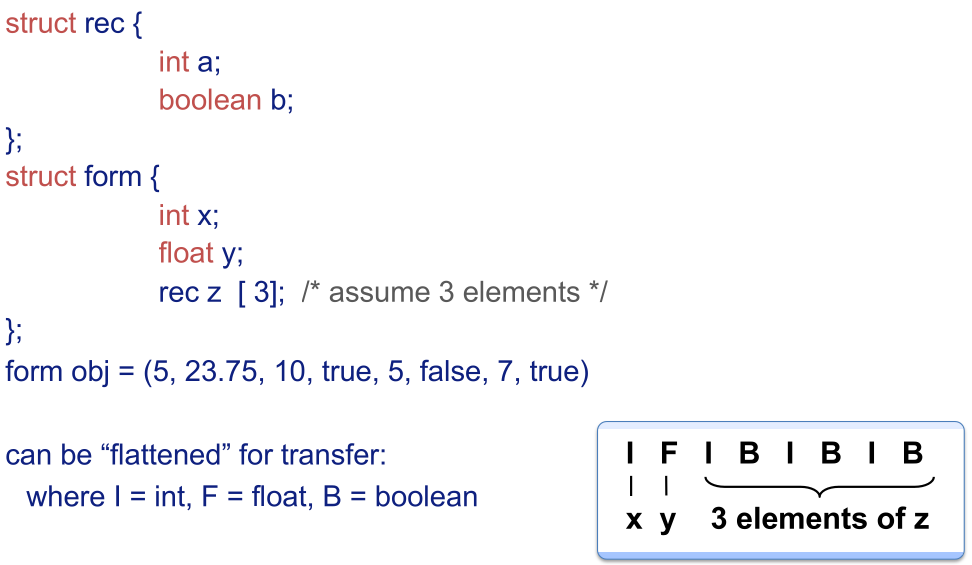
\includegraphics[scale=0.30]{composed_struct.png}
  	\centering
\end{figure}

\subsection{Object references(pointers)}
\quad

\begin{figure}[h]
  	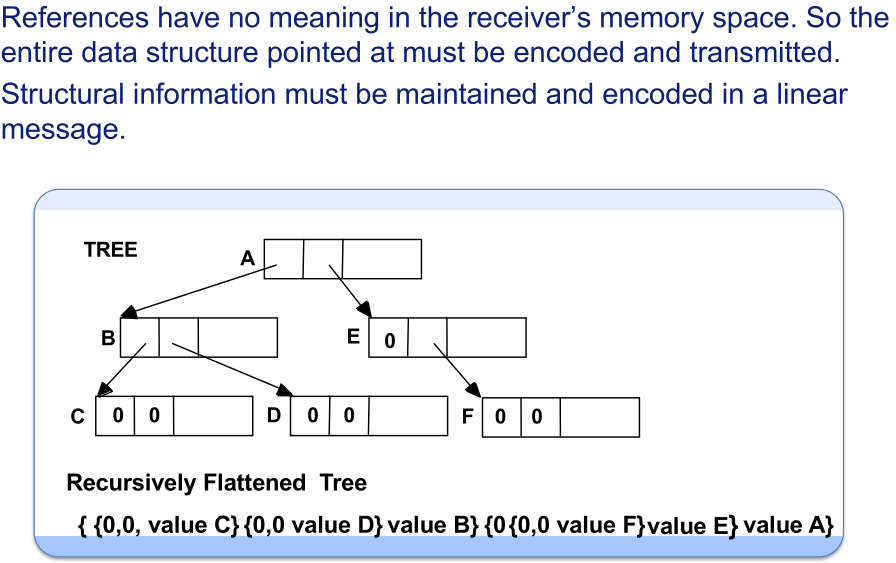
\includegraphics[scale=0.26]{obj_ref.png}
  	\centering
    \caption{Reference within the object}
\end{figure}

\begin{figure}[h]
  	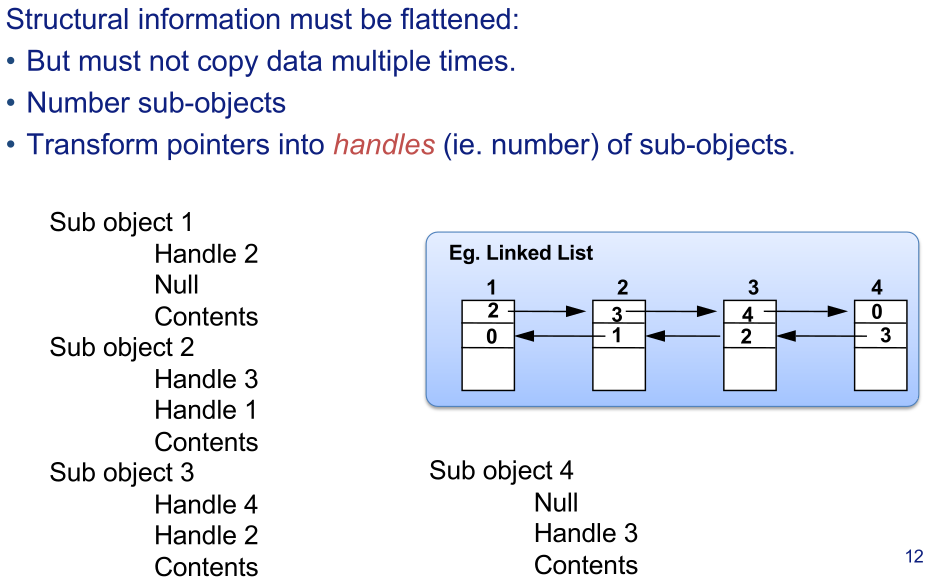
\includegraphics[scale=0.27]{ref_transmitted.png}
  	\centering
    \caption{Reference to objects already transmitted}
\end{figure}

\subsection{Extensible Markup Language (XML)}

\begin{itemize}
    \item \textbf{element}: container for data, enclosed by start and end tag.
        can contain other elements.
    \item \textbf{attribute}: used to label data --- usually name/value
    \item \textbf{namespace}: used to scope names
        \begin{itemize}
            \item defining a set of names each for a collection of 
                element types and attributes referenced by a url 
            \item specify namespace by \texttt{xmlns} attributes
            \item can use namespace name as prefix for names
        \end{itemize} 
    \item \textbf{schema}: defines elements and attributes that can appear in a
        document
\end{itemize} 

\begin{figure}[h]
  	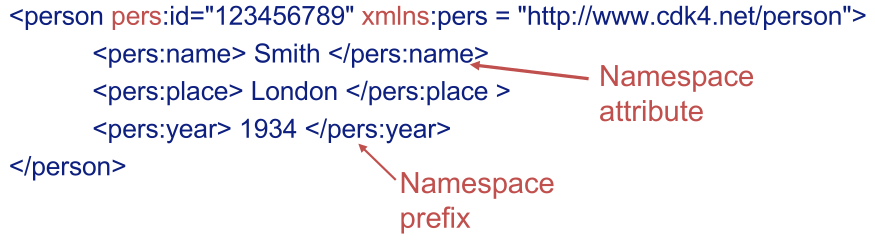
\includegraphics[scale=0.35]{xml.png}
  	\centering
    \caption{an example for XML}
\end{figure}

\begin{figure}[h]
  	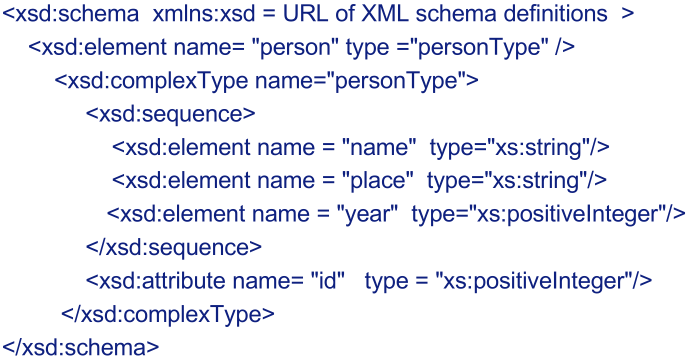
\includegraphics[scale=0.35]{xml_schema.png}
  	\centering
    \caption{an example for XML Schema}
\end{figure}


\subsection{JSON}

\begin{itemize}
    \item structural tokens: [ \{ ] \} : ,
    \item literal name tokens: \texttt{true}, \texttt{false}, \texttt{null}
    \item value: \texttt{object}, \texttt{array}, \texttt{number},
        \texttt{string}, \texttt{true}, \texttt{false}, \texttt{null}.
    \item object: \{ \texttt{string} : \texttt{value}, \texttt{string} : \texttt{value}, \ldots\}
    \item array: [ \texttt{value}, \texttt{value}, \ldots]
    \item string: ``\textlangle sequence of Unicode character\textrangle'' with usual escapes
\end{itemize} 

\begin{figure}[h]
  	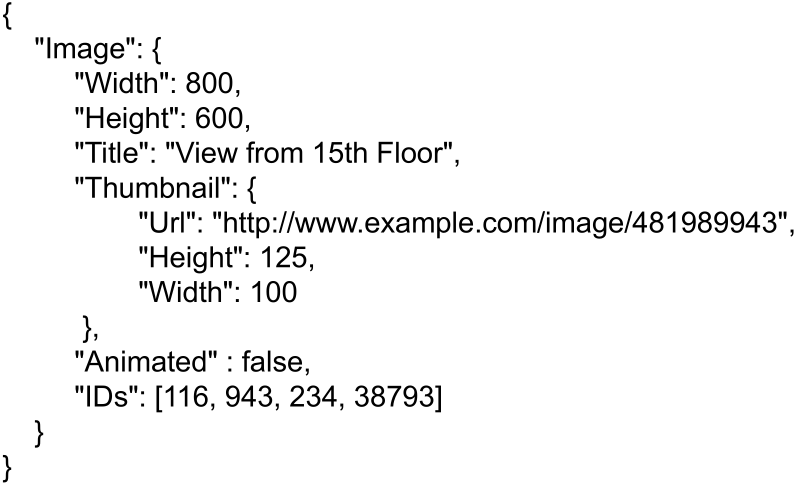
\includegraphics[scale=0.3]{JSON.png}
  	\centering
    \caption{an example for JSON}
\end{figure}


\subsection{Java Object Serialization}

\begin{itemize}
    \item Type (class) information is included with the serialization.
    \item Reference to other objects are treated as \emph{handles}.
    \item \textbf{Reflection}: the ability to query a class for the name and
        types of its attributes and methods
    \item Reflection allows for generic code for marshalling and unmarshalling.
    \item steps of serialization
        \begin{enumerate}
            \item write class information
            \item write types and names of instance variables
            \item if instance variables are of a new class, then repeat the
                above two steps for those variables
            \item uses serialization
        \end{enumerate} 
\end{itemize} 

\begin{figure}[h]
  	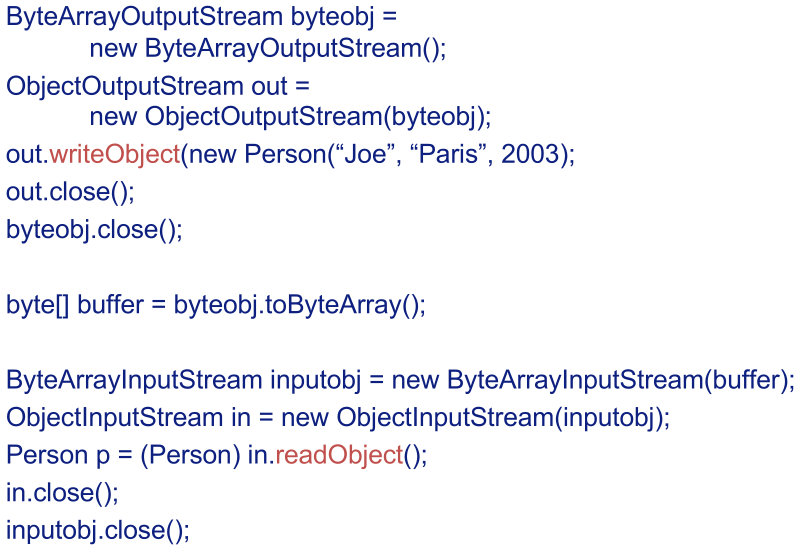
\includegraphics[scale=0.3]{java_serialization.png}
  	\centering
    \caption{an example for Java Object Serialization}
\end{figure}

\subsection{Liminations}

\begin{itemize}
    \item Representations can have similar syntax but different meaning
        \begin{itemize}
            \item e.g. rectangular or polar coordinates, transformation is
                application dependent
        \end{itemize} 
    \item Type may have no meaning outside own context
        \begin{itemize}
            \item e..g pointer, file name
        \end{itemize} 
    \item Procedures passed as parameters
        \begin{itemize}
            \item cannot always transfer code to different computer for
                execution
        \end{itemize} 
\end{itemize} 


\section{Remote Procedure Calls (RPCs)}

\subsection{RPC Interactions}

\begin{enumerate}
    \item Client is suspended until the call completes.
    \item Request must include name of the operation and parameters passed
        \emph{by value}.
    \item Server operates locally and sends the result (in one or
        multiple messages).
    \item Client decodes result and returns it to the calling procedure, which
        then continues processing.
\end{enumerate} 

\subsection{Stub Procedures}

\begin{itemize}
    \item Client-side definition: the implementation of encoding parameters,
        send request messages, wait for reply and decode the reply and return.
    \item Server-side definition: the implementation of receive request,
        identify local procedure, decode parameters, call the
        procedure, encode and send the result.
    \item what \textbf{stubs} do in general:
        \begin{itemize}
            \item parameter marshalling (packing)
            \item unmarshal (unpack) received messages and assign values to
                parameters
            \item transform data representations if necessary
            \item access communication primitives to send/receive messages.
        \end{itemize} 
    \item Stubs can be automatically generated from an \emph{interface
        specification}.
\end{itemize} 

\subsection{Dispatcher}

It maps incoming calls onto relevant procedure (stub).
Dispatcher at server receives all ``call'' messages and uses procedure
number (name) to identify called procedure.
Upon receiving requests from client, the server
\begin{enumerate}
    \item unmarshalls method object
    \item uses method info to unmarshall arguments
    \item converts remote object reference to local object reference
    \item calls method object's invoke method supplying local object reference
        and arguments
    \item when method executed, marshalls result or exceptions into reply
        message and sends it back to client
\end{enumerate} 

\subsection{Interface Compiler}
\begin{itemize}
    \item generates a number for each procedure in interface 
        -- inserted into call message by client stub procedure.
    \item generates the stub code and the skeleton code which can then
        be compiled with the client and the server.
    \item needs to be specified by the \textbf{Interface Definition
        Language (IDL)} to
        \begin{itemize}
            \item define the types that can be used
            \item define the interfaces and procedures that can be
                called
            \item define the direction of the parameters: in, out, inout
            \item mappings to specific languages
            \item e.g. the following
                \begin{figure}[h]
                    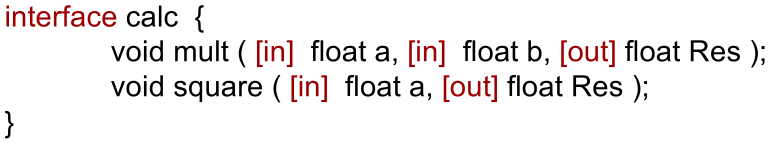
\includegraphics[scale=0.3]{IDL.png}
                    \centering
                \end{figure}
        \end{itemize} 
\end{itemize} 

\subsection{Interface Type Checking}

\subsubsection{Same Interface}

\begin{itemize}
    \item Identity can be specified, e.g.
        \begin{itemize}
            \item checksum over source
            \item name + timestamp of last modification or compilation
        \end{itemize} 
    \item  Client and server hold identity of interface.
    \item While connecting, check type identities are equal.
    \item This provides \textbf{strong type compatibility}.
\end{itemize} 

\subsubsection{Allow subtyping}

Permit server to be subtype of client interface, i.e.\ provides
additional operations which are not used by client, but must snot modify
operations in original interface.

\subsubsection{Structural Compability}

Maintain run-time representation of interface and check for structural
compatibility when client connects to server. The two interfaces shown in
Figure~\ref{fig:wtc} are structurally equivalent. This provides \textbf{weak
type compatibility}.

\begin{figure}[h]
  	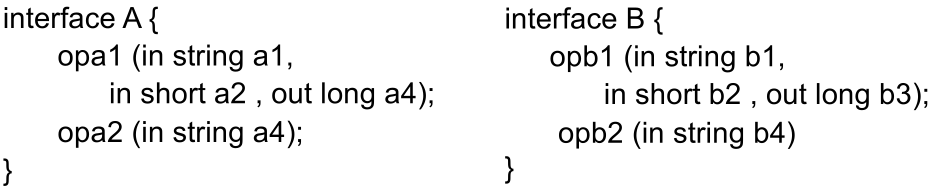
\includegraphics[scale=0.35]{weak_type_compatibility.png}
  	\centering
    \caption{weak type compatibility example}\label{fig:wtc}
\end{figure}


\subsection{Binding}

\begin{itemize}
    \item definition:
        \begin{itemize}
            \item connecting to a specific server
            \item assignment of a reference value (e.g. address or object
                reference) to a placeholder (e.g. message port or object
                reference variable)
        \end{itemize} 
    \item \textbf{Name server} (or \textbf{directory server}) is used to
        register exported interfaces and is queried to locate a server when an
        interface is imported.
        \begin{itemize}
            \item When a server starts it \emph{exports} a reference to the
                interface to the name server.
            \item When a client wants to use a service it connects to the name
                server and \emph{imports} a reference to the server.
        \end{itemize} 
    \item Please refer to the coursework code to see how Java RMI binds client
        with server.
\end{itemize} 

\subsection{Failure}

\subsubsection{Best Effort (Maybe) semantics}

As shown in the following, there is \emph{no fault tolerance measures}.

\begin{figure}[h]
  	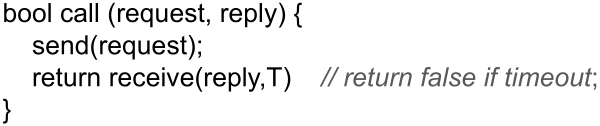
\includegraphics[scale=0.35]{maybe_semantics.png}
  	\centering
\end{figure}
\noindent The semantics is lightweight, but leaves issues of state consistency of the
server, with repsect to the client, up to the application programmer.


\subsubsection{At least once semantics}

As shown in the following, retries up to $n$ times 
--- if the call succeeds then procedure has been
executed once or more times since duplicate messages may have been generated.

\begin{figure}[h]
  	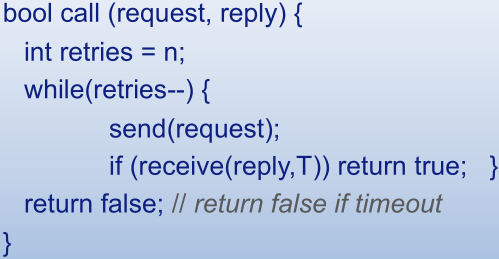
\includegraphics[scale=0.27]{ato_semantics.png}
  	\centering
\end{figure}

\noindent This is useful for \textbf{idempotent} server operations, i.e.\ multiple
executions leave the same effect on server state as a single execution.


\subsubsection{At most once semantics}

\begin{itemize}
    \item Guarantees that the remote procedure is either not executed or
        executed once.
    \item The server must 
        \begin{itemize}
            \item keep track of request identifiers and discard 
                retransmitted requests that have not completed execution.
            \item buffer replies and retransmit until acknowledged by the client.
            \item not crash to guarantee at-most-once semantics
        \end{itemize} 
    \item It effectively achieves exactly-once semantics if no errors or
        exceptions have occurred.
\end{itemize} 

\begin{figure}[h]
  	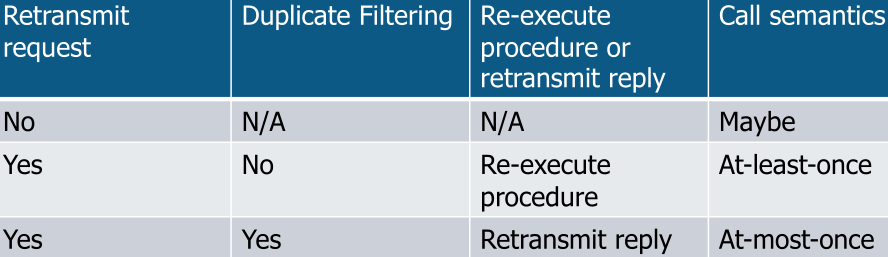
\includegraphics[scale=0.35]{semantics.png}
  	\centering
  	\caption{Failure semantics comparison}
\end{figure}

\subsubsection{Zero or once (Transactional) semantics}

\begin{itemize}
    \item Guarantees that either the procedure is completely executed or it is
        not executed at all.
    \item The server must implement an \emph{atomic transaction for each RPC}.
        \begin{itemize}
            \item either the state data in the server is updated permanently by
                an operation taking it from one consistent state to another
            \item or it is left in its original state, if the call is aborted or
                a failure occurs.
        \end{itemize} 
    \item This requires ACID (Atomicity, Consistency, Isolation, Durability)
        properties and implemented by a \emph{two-phase commit} type of
        protocol.
        \begin{itemize}
            \item phase 1: prepares all the aspects of the transaction
            \item phase 2: permanently commit or abort them
        \end{itemize} 
\end{itemize} 

\subsubsection{Server Failure}

\begin{itemize}
    \item Client needs to know server epochs to know if there is server failure
        leading to loss of state information in the server.
    \item Use \texttt{exportid} to detect failed server: when server restarts a
        new \texttt{exportid} is generated and exported.
    \item Client receives \texttt{exportid} during binding and will include it
        in all messages to the server.
    \item Dispatcher aborts calls with incorrect \texttt{exportid}.
\end{itemize} 

\subsubsection{Client Failure}

\begin{itemize}
    \item \textbf{Orphan executions}: result from a client crashing while the
        server is executing the procedure.
    \item Server's response will then not be acknowledged. Server either
        implements a form of rollback or does nothing.
    \item For long running procedures, to avoid wasting resources, the server
        may wish to be informed of client crashes so that it can abort orphan
        executions.
\end{itemize} 


\subsection{Implementation}

\begin{itemize}
    \item \textbf{TID}: a \emph{transaction identifier} for each invocation. This
        includes the export identifier.
    \item \textbf{sn}: a message \emph{sequence number} to detect duplicate
        messages and messages which follow in the sequence of invocations.
    \item \textbf{flag}:
        \begin{itemize}
            \item \texttt{ack}: please acknowledge message
            \item \texttt{no ack}: no acknowledgement expected
        \end{itemize} 
    \item \textbf{params}: in or out parameters as needed.
    \item Please see Figure~\ref{fig:rpc} for an example of RPC implementation.
\end{itemize} 

\begin{figure}[h]
  	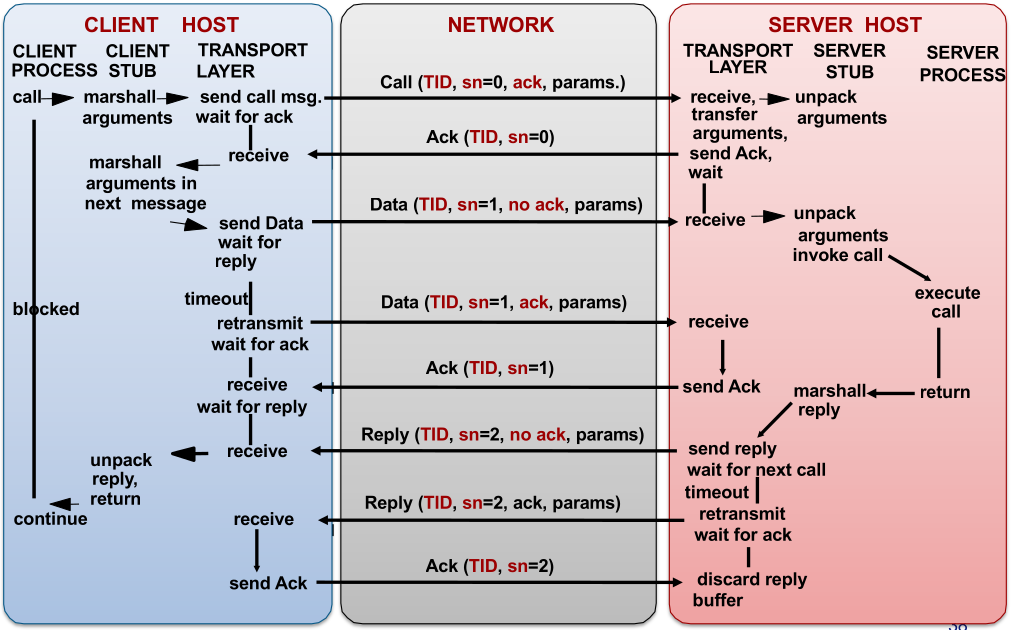
\includegraphics[scale=0.33]{rpc_impl.png}
  	\centering
  	\caption{An example of RPC implementation}\label{fig:rpc}
\end{figure}

\subsection{Concurrency}

\begin{itemize}
    \item client: no deadlocks with \emph{callbacks} if client multi-threaded.
    \item server:
        \begin{itemize}
            \item \underline{thread-per-request}: dispatcher creates new thread to handle
                each request
            \item \underline{thread pool}: fixed number of threads generated at start-up,
                free threads are allocated to requests by the dispatcher. lower
                creation overhead.
            \item \underline{thread-per-session}: a thread is created at connection set up
                to process all requests from the particular client.
        \end{itemize} 
\end{itemize} 


\section{Distributed Object Systems (Java RMI)}

\subsection{Remote Interface}

\begin{figure}[!bh]
  	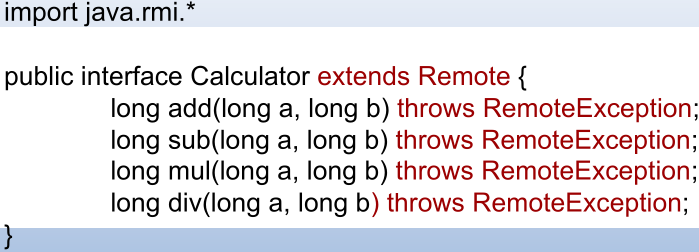
\includegraphics[scale=0.32]{RMI_interface.png}
  	\centering
    \caption{An example of remote interface}
\end{figure}

\subsection{Client Server Interaction}

\begin{itemize}
    \item relies on the ability to dynamically load code i.e.\ stub.
    \item skeleton not needed in later versions of java.
\end{itemize} 

\begin{figure}[h]
  	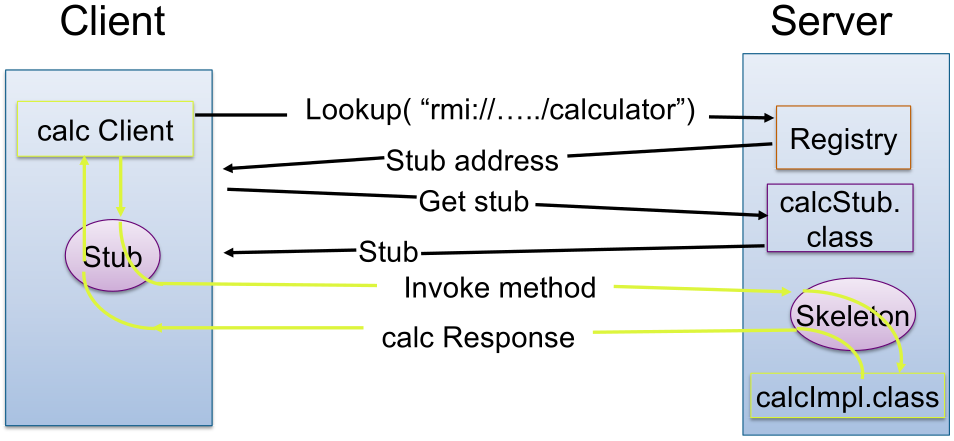
\includegraphics[scale=0.30]{RMI_interaction.png}
  	\centering
    \caption{An example of client-server interaction}
\end{figure}

\subsection{Remote Object Implementation}

An object is implicitly \emph{exported} if its class derives from the class
\texttt{java.rmi.server.UnicastRemoteObject}.

\begin{figure}[!h]
  	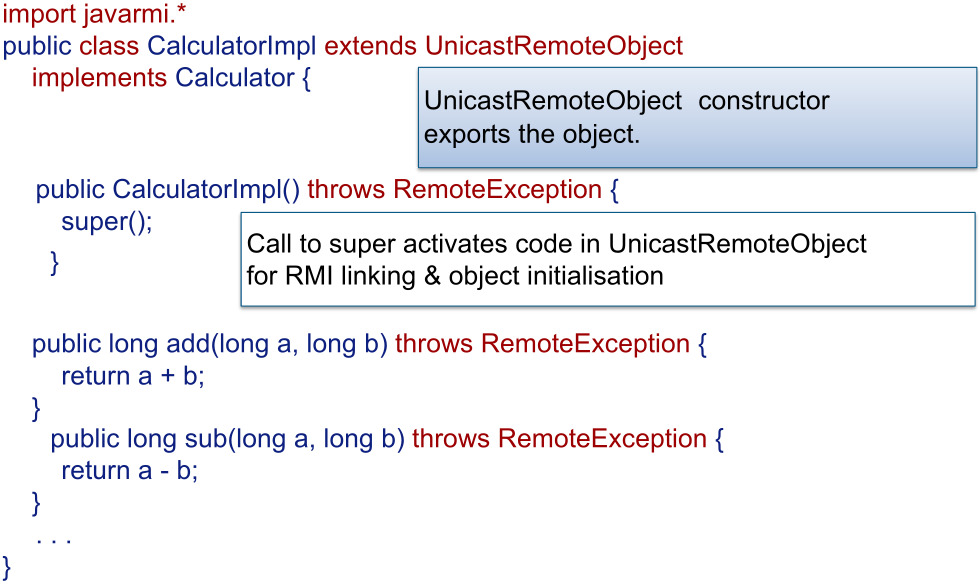
\includegraphics[scale=0.30]{remote_obj.png}
  	\centering
    \caption{An example of remote object implementation}
\end{figure}

\subsection{Server and Client Implementation}

\begin{itemize}
    \item A server creates remote objects as part of mainline code.
    \item A server may advertise references to objects it hosts via
        RMI registry.
    \item Registry allows a binding between a URL for an object and an object
        reference to be queried by potential clients.
        \begin{itemize}
            \item An object's name is a URL formatted as ``//host:port/name''.
            \item Both host and port are optional.
        \end{itemize} 
    \item The server listens for incoming invocation requests which are
        dispatched to appropriate object.
    \item RMI security manager is needed in server and client if stub is loaded
        from server.
        \begin{itemize}
            \item check if various operations performed by a stub are allowed 
            \item e.g. access to communications, files, control virtual machine,
                etc.
        \end{itemize} 
\end{itemize} 

\begin{figure}[h]
  	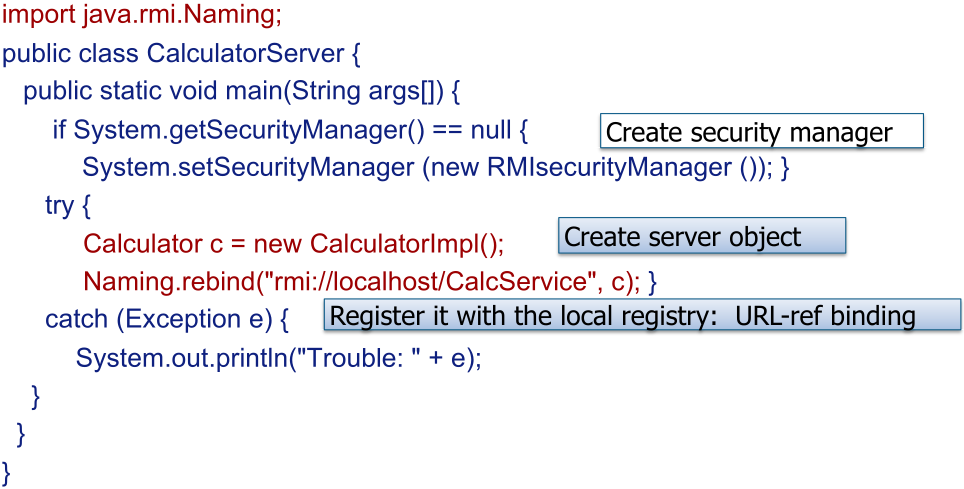
\includegraphics[scale=0.30]{server.png}
  	\centering
    \caption{An example of server implementation}
\end{figure}

\begin{figure}[h]
  	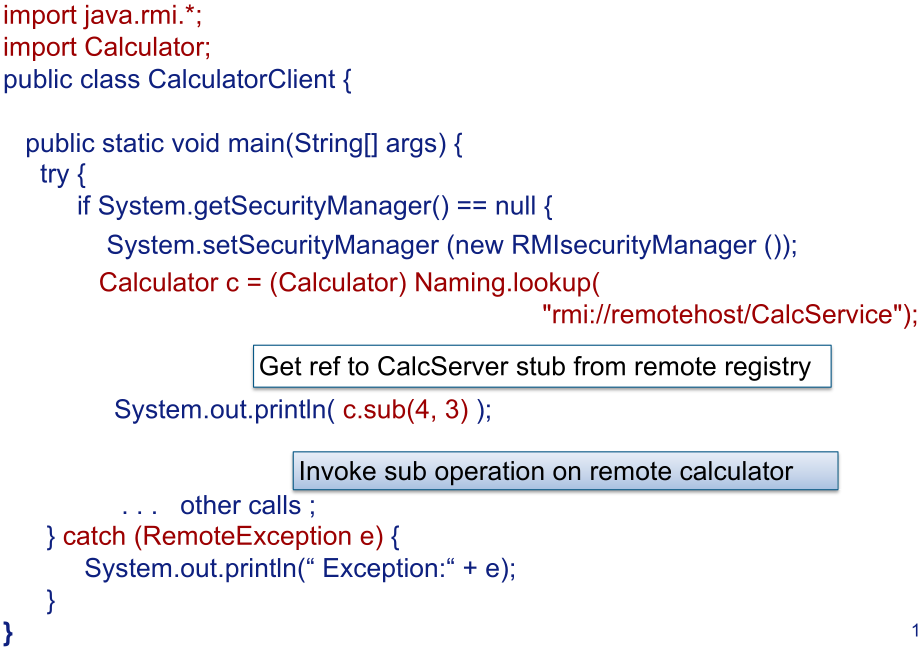
\includegraphics[scale=0.30]{calc_client.png}
  	\centering
    \caption{An example of calculator client implementation}
\end{figure}

\subsection{Garbage Collection of Remote Objects}

RMI runtime system automatically deletes objects no longer referenced by a
client.
\begin{itemize}
    \item When live reference enters Java VM, its reference count is incremented
    \item First reference sends ``referenced'' message to server
    \item After last reference discarded in client, ``unreferenced'' message
        sent to server.
    \item Remote object removed when no more local or remote references exist.
\end{itemize} 


\section{Time Service}

\subsection{Cristian's Algorithm}

\begin{figure}[h]
  	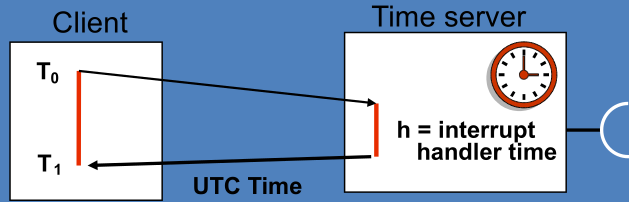
\includegraphics[scale=0.35]{cristian.png}
  	\centering
\end{figure}

\begin{itemize}
    \item Assume reference time server with UTC time.
    \item estimated message propoagation time 
        \[
            p=\frac{T_1-T_0-h}{2}
        \]
    \item set clock to UTC + $p$, where UTC is the time received from the
        server
    \item Measure $T_1-T_0$ over several transactions, \emph{remove outliers}
        and/or \emph{take minimum values} as being most accurate as smaller
        network delays.
    \item[-] Single server would be bottleneck, a single point of failure or a
        single point of compromise.
\end{itemize} 

\subsection{Berkley Algorithm}

\begin{figure}[h]
  	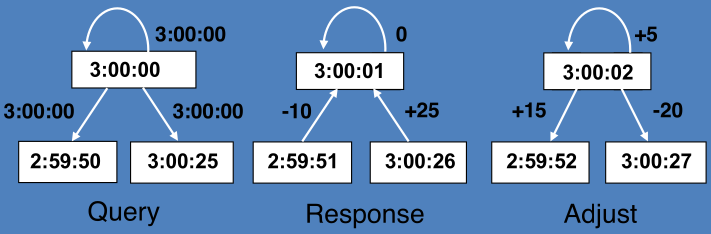
\includegraphics[scale=0.35]{berkley.png}
  	\centering
\end{figure}

\begin{enumerate}
    \item Query: \textbf{Coordinator}, chosen as master, periodically polls slaves to
        query clocks.
    \item Response: estimates local times with compensation for propagation
        delay and calculates average time but ignores outliers e.g. large
        propagation delay
    \item Adjust: sends message to each slave indicating clock adjustment.
\end{enumerate} 

\subsection{Network Time Protocol (NTP)}

\begin{itemize}
    \item Synchronize large number of computers
    \item Organize servers in \textbf{strata}.
        \begin{figure}[h]
            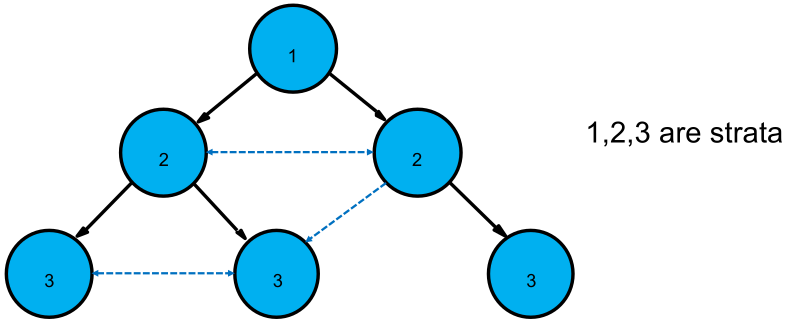
\includegraphics[scale=0.30]{strata.png}
            \centering
        \end{figure}
    \item Multiple servers across the Internet connected to UTC receivers
        (\textbf{primaries}). 
    \item \emph{Secondary} servers synchronize with primaries.
    \item \emph{Tertiary} servers synchronize with secondary servers etc.
    \item synchronization modes
        \begin{itemize}
            \item broadcast/multicast: one or more servers periodically
                multicast to other computers on \emph{high speed LAN}. Assume
                small delay.
            \item procedure-call/client-server: a client requests time from a
                few other servers, similar to \underline{Critstian's algorithm}.
            \item symmetric: used by master servers on LANs and layers closest
                to primaries, higher accuracy based on pairwise synchronization.
                \begin{figure}[h]
                  	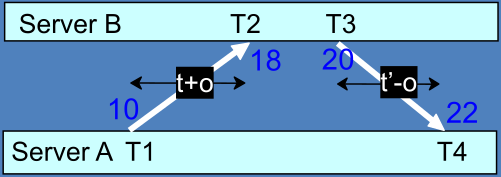
\includegraphics[scale=0.30]{symmetric.png}
                  	\centering
                  	\caption{an example of NTP symmetric protocol}\label{fig:sym}
                \end{figure}
                \begin{itemize}
                    \item Using the example in Figure~\ref{fig:sym}, with $t$
                        and $t'$ being the transmission delay, and $o$ being the
                        clock offset of $B$ relative to $A$,
                        let $a=T_2-T_1=t+o$, $b=T_4-T_3=t'-o$, we have
                        \[
                            \text{RTT} = t + t' = a + b = (T_2-T_1)+(T_4-T_3)
                        \]
                        and 
                        \[
                            2o=a-b=(T_2-T_1)-(T_4-T_3)
                        \]
                        assuming $t=t'$.
                \end{itemize} 
        \end{itemize} 
\end{itemize} 

\subsection{Vector Clocks}

\begin{itemize}
    \item Logical clocks are sufficient for causal ordering.
    \item $V_i[j]$ indicates the logical clock of process $j$ known by
        process $i$.
    \item just before timestamping an event, $++V_i[i]$.
    \item when it receives a timestamp $t$ in a message, set
        \[
            V_i[j]=\text{max}(V_i[j],t[j]), 
            \quad\forall
            j\in\left\{1,2,\ldots,N\right\}.
        \]
        \begin{figure}[h]
          	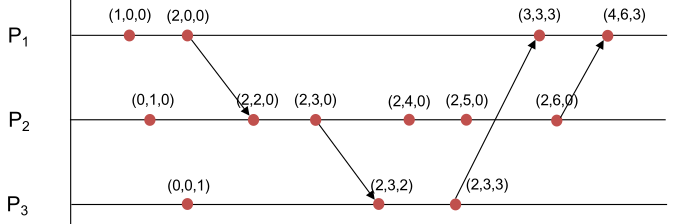
\includegraphics[scale=0.35]{vector_clock.png}
          	\centering
        \end{figure}
        
    \item we then have
        \begin{itemize}
            \item if $a$ is the event of a message $m$ being sent from process
                $A$ and $b$ is the event of $m$ being received by process $B$
                then $a\rightarrow b$.
            \item $a\rightarrow b \iff V(a)\le V(b)$.
            \item if neither $V(a)\le V(b)$ nor $V(a)\ge V(b)$, $a$ and $b$ are
                concurrent.
        \end{itemize} 
    \item We can define a \textbf{consistent cut} accross the history of events, 
        where the causes are present for all the effects.
\end{itemize} 


\section{Coordination}

\begin{itemize}
    \item \textbf{Synchronous system} means that maximum bounds can be put on:
        transmission delay, clock drift rate, time taken to execute an action.
        This means that we can detect when something has not happened.
    \item \textbf{Asynchronous system} means that no timing assumptions can be
        made. A message can take indefinite time to arrive and thus cannot
        distinguish between a failure and a long-term process.
\end{itemize} 

\subsection{Unreliable v.s. Reliable Failure Detectors}

\begin{itemize}
    \item \underline{Unreliable failure detector} is not necessarily accurate,
        and tells whether a process is \emph{suspected}/\emph{unsuspected} 
        to have failed.
    \item \underline{Reliable failure detector} \emph{determines} 
        whether a process has (not) failed.
        If failed, not process recovery is considered.
    \item e.g. say process $P_1$ sends ``$P_1$ alive'' message to all other
        process every $T$ seconds
        \begin{itemize}
            \item Failure detector at each process estimates \emph{maximum}
                message transmission time $D$.
            \item choice of $T$ should reflect network delay condition
            \item Expects a message every $T+D$ seconds --- if received, ok; if
                not, suspects $P_1$ failed.
            \item For \underline{asynchronous} system, this is
                \underline{unreliable}; for \underline{synchronous} system, this
                is \underline{reliable}.
        \end{itemize} 
\end{itemize} 

\subsection{Mutual Exclusion}

\subsubsection{Properties and Performance}

\subsubsubsection{Properties}

\begin{itemize}
    \item \textbf{Safety}: at most one process enters the critical section
    \item \textbf{Liveness}: requests eventually succeed, no process is blocked
        forever
    \item \textbf{Fairness}: requests are satisfied in some order in
        which they are sent
\end{itemize} 

\noindent\subsubsubsection{Performance}

\begin{itemize}
    \item minimize the bandwidth, e.g. number of messages required
    \item minimize synchronization delay, i.e.\ between one acccess and the
        following one.
\end{itemize} 

\subsubsection{Central Server Algorithm}

\begin{enumerate}
    \item Processes request access from central server
    \item Server replies with access token, when access is granted. Other
        requests are queued.
    \item Processes release token on finishing access.
\end{enumerate} 

\subsubsubsection{Properties}

\begin{itemize}
    \item Safety is satisfied.
    \item Liveness is satisfied if each request is bounded.
    \item Fairness is not satisfied.
\end{itemize} 

\subsubsubsection{Performance}

\begin{itemize}
    \item 3 messages required for each request.
    \item 1 RTT required for synchronization delay. Release + Token message need
        to be sent.
\end{itemize} 

\subsubsubsection{Comments}

\begin{itemize}
    \item simple
    \item central point of failure/central bottleneck
    \item must have a desginated (or elected) server
\end{itemize} 

\subsubsection{Ring-based Algorithm}

\begin{itemize}
    \item remove central server
    \item processes pass token to each other in a ring, i.e.\ when finished
        $p_i$ sends token to $p_{i+1(\text{mod}\;n)}$.
    \item When a token is received by a process
        \begin{itemize}
            \item it uses the token if it requires it
            \item it passes the token if it doesn't
        \end{itemize} 
\end{itemize} 

\subsubsubsection{Properties}

\begin{itemize}
    \item Safety is satisfied.
    \item Liveness is satisfied if each request is bounded.
    \item Fairness: not in order of requests.
\end{itemize} 

\subsubsubsection{Performance}

\begin{itemize}
    \item Delay to access between 0 and $N$ messages.
    \item Synchronization delay between 1 and $N$ messages.
    \item Uses messages even if no one wants to use the resource.
\end{itemize} 

\subsubsubsection{Comments}

\begin{itemize}
    \item Variant is to embed the request time in the token and pass on tokens
        with earlier request times.
    \item Any failure breaks the ring. Needs procedures to cope with token loss
        and process failure in the general case.
\end{itemize} 

\subsubsection{Ricart \& Agrawala}

Please see Figure~\ref{fig:ricart} for the detail.

\begin{figure}
  	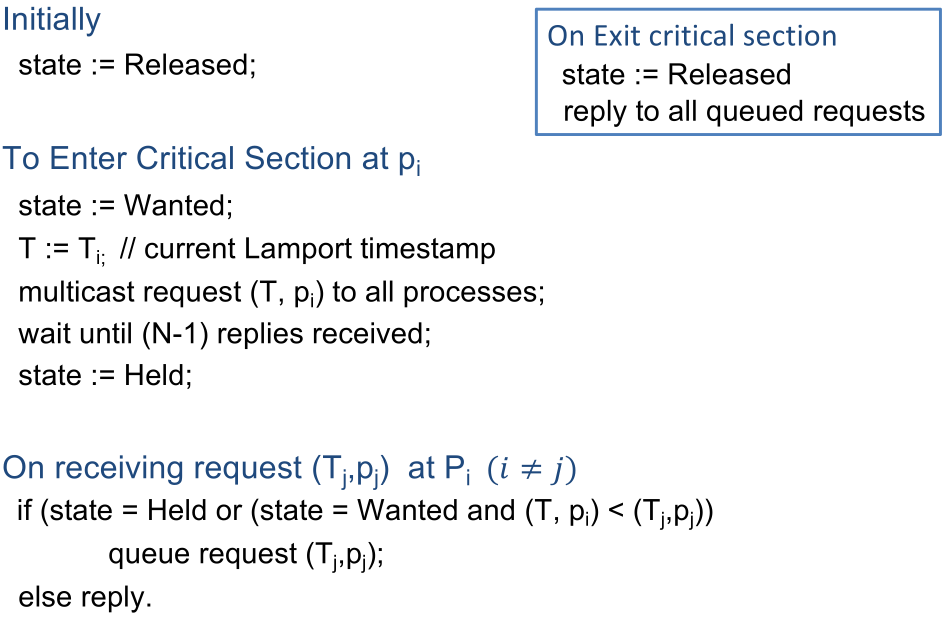
\includegraphics[scale=0.30]{ricart.png}
  	\centering
    \caption{Ricart \& Agrawala's algorithm}\label{fig:ricart}
\end{figure}

\subsubsubsection{Properties}

\begin{itemize}
    \item Safety: mutual requests are \emph{totally ordered} so only one will
        receive all replies.
    \item Liveness: eventually all processes will release
    \item Fairness: order of Lamport logical timestamps
\end{itemize} 

\subsubsubsection{Performance}

\begin{itemize}
    \item gaining entry requires: $N-1$ replies and 1 (if multicast support) or
        $N-1$ (if no multicast support messages).
    \item minimum synchronization delay: 1 message
\end{itemize} 

\subsubsubsection{Comments}

Highly dependent on reliability of processes and messages.


\subsection{Elections}

\begin{enumerate}
    \item Set of processes $p_i$, each has a variable $\texttt{elected}_i$.
    \item Processes can be \texttt{participant} or \texttt{non-participant}.
    \item At the beginning of the election all participants set
        $\texttt{elected}_i=\texttt{null}$.
    \item At the end of election, all particpant processes must have the same
        value e.g. $P$ of $\texttt{elected}_i$.
\end{enumerate} 

\subsubsection{Ring Elections}

\subsubsubsection{Steps}

\begin{enumerate}
    \item Initially all $P_i$ are nonparticipants.
        \begin{itemize}
            \item $P_i$ calls for election
            \item $P_i^\text{status}:=\text{part(participant)}$.
            \item send \texttt{election($P_i$)} to $P_{i+1\mod{n}}$
        \end{itemize} 
    \item When $P_j$ receives \texttt{election(ident)}:
        \begin{itemize}
            \item (First Round) if $\texttt{ident}>P_j$: 
                forward \texttt{election(ident)},
                set $P_j^\text{status}:=\texttt{part}$.
            \item (Second Round) if $\texttt{ident}<P_j\wedge
                P_j^\text{status}=\texttt{nonpart}$:
                send \texttt{election($P_j$)}, 
                set $P_j^\text{status}:=\texttt{part}$.
            \item (Third Round) if $\texttt{ident}=P_j$:
                send \texttt{elected($P_j$)},
                $P_j^\text{status}=\texttt{nonpart}$.
        \end{itemize} 
    \item When $P_j$ receives \texttt{elected(ident)}:
        \begin{itemize}
            \item $\texttt{elected}_j=\texttt{ident}$,
                $P_j^\text{status}:=\texttt{nonpart}$.
            \item foward \texttt{elected(ident)}, \emph{unless}
                $\texttt{ident}=P_j$.
        \end{itemize} 
\end{enumerate} 

\subsubsubsection{Analysis}

\begin{itemize}
    \item Assumptions: No failures, asynchronous, any process can begin an election.
    \item Safety \& liveness: eventually all processes will receive and agree on
        the maximum if there are no failures.
    \item Performance: worst case $3N-1$ messages required for single election.
\end{itemize} 

\subsubsection{Bully}

\subsubsubsection{Steps}

\begin{enumerate}
    \item When $P_i$ notices the coordinator is no longer there it initiates an
        election by sending `ELECTION' to all $P_j$ with $j>i$.
    \item There are two cases:
        \begin{itemize}
            \item If no `ANSWER' received, it declares itself as the
                `COORDINATOR'.
            \item If `ANSWER' received, it waits for a `COORDINATOR' message. If
                non arrives, it starts a new election. If arrives, it sets
                $\texttt{elected}_i$ to the value received.
        \end{itemize} 
    \item When $P_j$ receives `ELECTION' it sends `ANSWER' and starts another
        election, unless it has already done it.
\end{enumerate} 

\begin{figure}
  	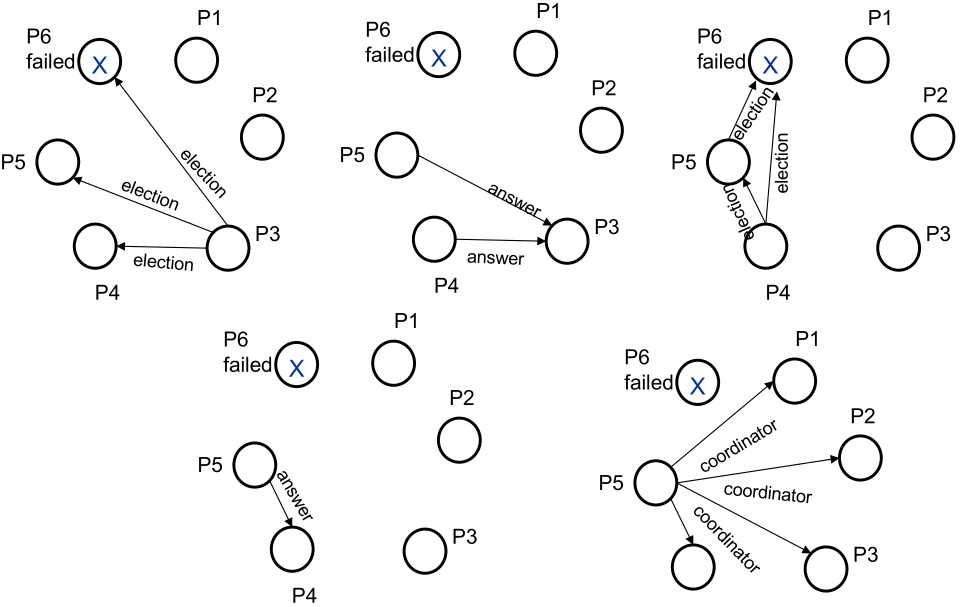
\includegraphics[scale=0.30]{bully.png}
  	\centering
  	\caption{An example of Bully election}
\end{figure}

\subsubsubsection{Analysis}

\begin{itemize}
    \item Safety: No two processes can decide that they are the coordinator,
        assuming that failed processes cannot be restarted with the same
        identifier. Otherwise two processes can start again and each decide that
        they are the coordinator.
    \item Liveness: If no messages are lost all available processes will reply.
    \item Performance: $O(N^2)$ in the worst case.
\end{itemize} 


\subsection{Consensus}

\subsubsection{The Byzantine General Problem}

A commanding general must send an order to his $n-1$ lieutenant generals s.t.
\begin{itemize}
    \item[IC1] All loyal lieutenants obey the same order.
    \item[IC2] If the commanding general is loyal, then every loyal lieutenant
        obeys the order he sends.
\end{itemize} 
where ``IC'' stands for Integrity Condition.
In the world of networks, command general can be mapped to the process sending
the request, lieutenants can be mapped to the receiving processes.

\begin{figure}[h]
  	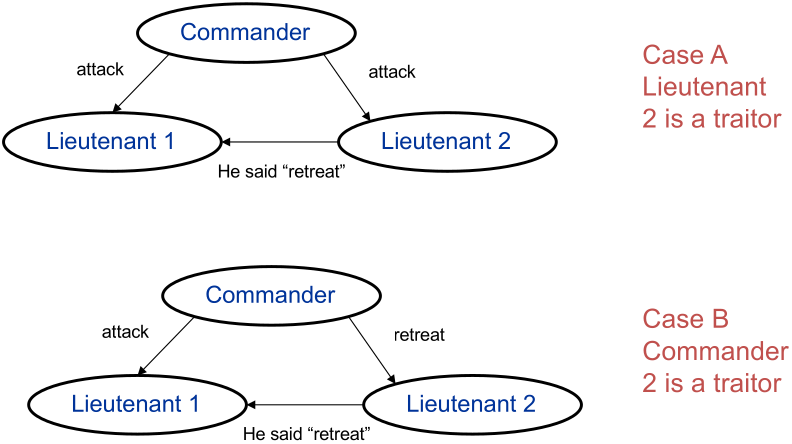
\includegraphics[scale=0.35]{byzantine.png}
  	\centering
    \caption{impossibility results}\label{fig:byz}
\end{figure}

From Figure~\ref{fig:byz}, we can see that in case B, if lieutenant 1 attacks
he violates IC1. Lieutenant 1 cannot distinguish, from the information available
to him, between case A \& case B.

\emph{No Solution exists for three generals that works in the presence of a
single traitor}.

\emph{In general, No solution with fewer than $3m+1$ generals can cope with $m$
traitors}.

\subsubsection{Unsigned Messages (UM)}

We define UM($n,m$) as the unsigned messages algorithm for $n$ generals and $m$
traitors, and assume that
\begin{itemize}
    \item every message that is sent is delivered correctly
    \item the receiver of a message knows who sent it
    \item the absence of a message can be detected
\end{itemize} 

\medskip\noindent
\subsubsubsection{UM($n,0$), i.e.\ no traitors}

\begin{itemize}
    \item Commander sends $v$ to every lieutenant
    \item Each lieutenant uses the value received or $v_\text{default}$ if no
        value received.
\end{itemize} 

\begin{figure}[h]
  	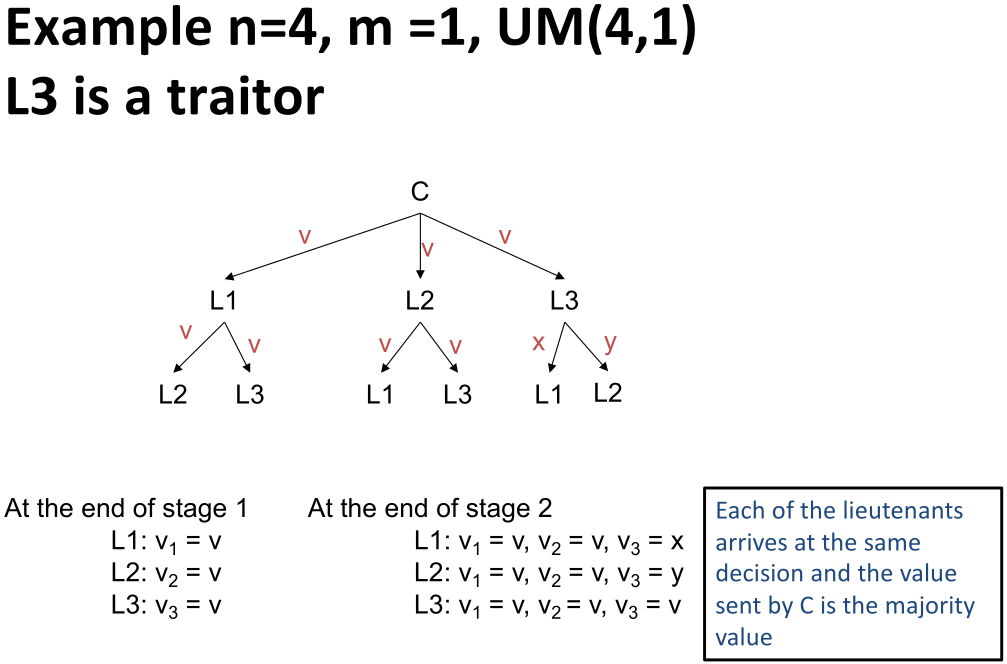
\includegraphics[scale=0.30]{L3.png}
  	\centering
\end{figure}

\noindent
\subsubsubsection{UM($n,m$)}

\begin{itemize}
    \item For each lieutenant,
        \begin{itemize}
            \item let $v_i$ be the value received from commander or
                $v_\text{default}$ if no value received
            \item send $v_i$ to $n-2$ other lieutenants using UM($n-1,m-2$)
        \end{itemize} 
    \item For each $i$ and each $j\neq i$
        \begin{itemize}
            \item let $v_i$ be the value lieutenant received from other
                lieutenants or $v_\text{default}$ if no value received.
            \item $\text{Lieutenant}_i$ uses majority($v_1,v_2,\ldots,v_{n-1}$).
        \end{itemize} 
\end{itemize} 
\begin{figure}[h]
  	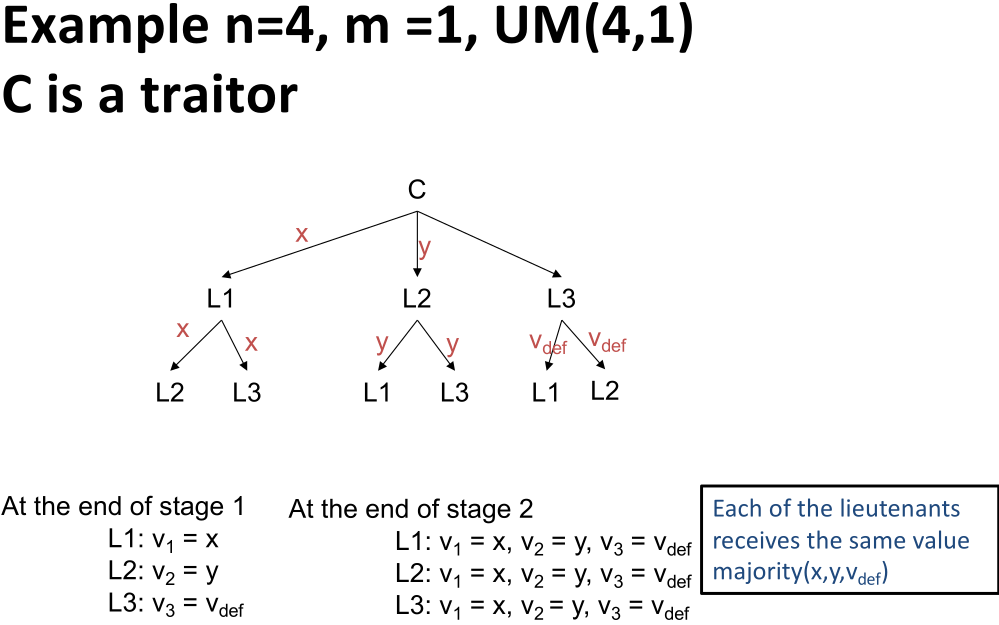
\includegraphics[scale=0.30]{C.png}
  	\centering
\end{figure}


\section{Security}

\subsection{Introduction}

\subsubsection{Goals}

\begin{itemize}
    \item \textbf{Confidentiality}: prevent disclosure of info to unauthorized users +
        prevent analysis of traffic characteristics
    \item \textbf{Integrity}: prevent modification of info by unauthorized users ---
        include no duplication, replays, insertions or reordering
    \item \textbf{Availability}: prevent denial of service e.g. by disruption
\end{itemize} 

\subsubsection{Requirements}

\begin{itemize}
    \item \textbf{Identification}: establishing the identity of the subject
    \item \textbf{Authentication}: validity of the identity of sender or server,
        e.g. passwords, biometrics, 2-factor authentication, etc.
    \item \textbf{Access control}: control over who has access to services or resources
        within the system.
\end{itemize} 

\subsection{Cryptography}

\subsubsection{Definition}

\begin{itemize}
    \item \textbf{Encryption}: a transformation of information based on
        substitution (table lookup) or transposition (exchanges bytes), i.e.\ a
        function $E$ with key $k$,
        \[
            E_k[M]
        \]
        where $M$ is the message.
    \item \textbf{Decryption}: inverse of encryption to obtain original
        information, i.e.\ a function $D$ with key $k'$,
        \[
            D_{k'}[C]
        \]
        where $C$ is the encrypted message.
\end{itemize} 

\subsubsection{Secret Key (Symmetric) Cryptography}

\begin{itemize}
    \item basis for \emph{Data Encryption Standard} (DES)
    \item $E=D$ and $k=k'$
\end{itemize} 

\subsubsection{Public Key (Asymmetric) Cryptography}

\begin{itemize}
    \item \textbf{Public key} ($K$) sent out over network and stored with name
        servers --- used by sender for encryption
    \item \textbf{Private key} ($K^{-1}$) used by recipient for decryption
    \item cannot deduce $K^{-1}$ from $K$
\end{itemize} 


\end{document}
